{\color{oorange}\subsection{Metodo del Gradiente implementato con ricerca in linea inesatta (backtracking)}}
Il metodo del gradiente è un algoritmo che cerca di trovare l'argomento del minimo globale, ovvero:
un vettore $x^{\ast}$ è un punto di minimo globale di $f(x)$ se $f(x^{\ast}) \leq f(x) \forall x \in R^n$.

Analogamente, un vettore $x^{\ast}$ è un punto di minimo globale in senso stretto di $f(x)$ 
se $f(x^{\ast}) < f(x) \forall x \in R+n \and x \neq x^{\ast}$.

In termini molto generali si può dire che la ricerca in linea esatta è finalizzata essenzialmente, ad assicurare 
la convergenza globale dell'algoritmo, mentre la rapidità di convergenza dipende in prevalenza dalla direzione 
di ricerca. 

Tuttavia, un valore di $a_k$ poco appropriato può distruggere le proprietà di rapidità di convergenza associate 
alla scelta di $p_k$.

Per questi motivi, anzichè fissare fin dall'inizio $\alpha$, ad ogni iterazione calcoliamo il passo più opportuno 
(ricerca in linea inesatta).

\begin{figure}[H]
    \centering
    \begin{subfigure}{0.9\textwidth}
        \centering
    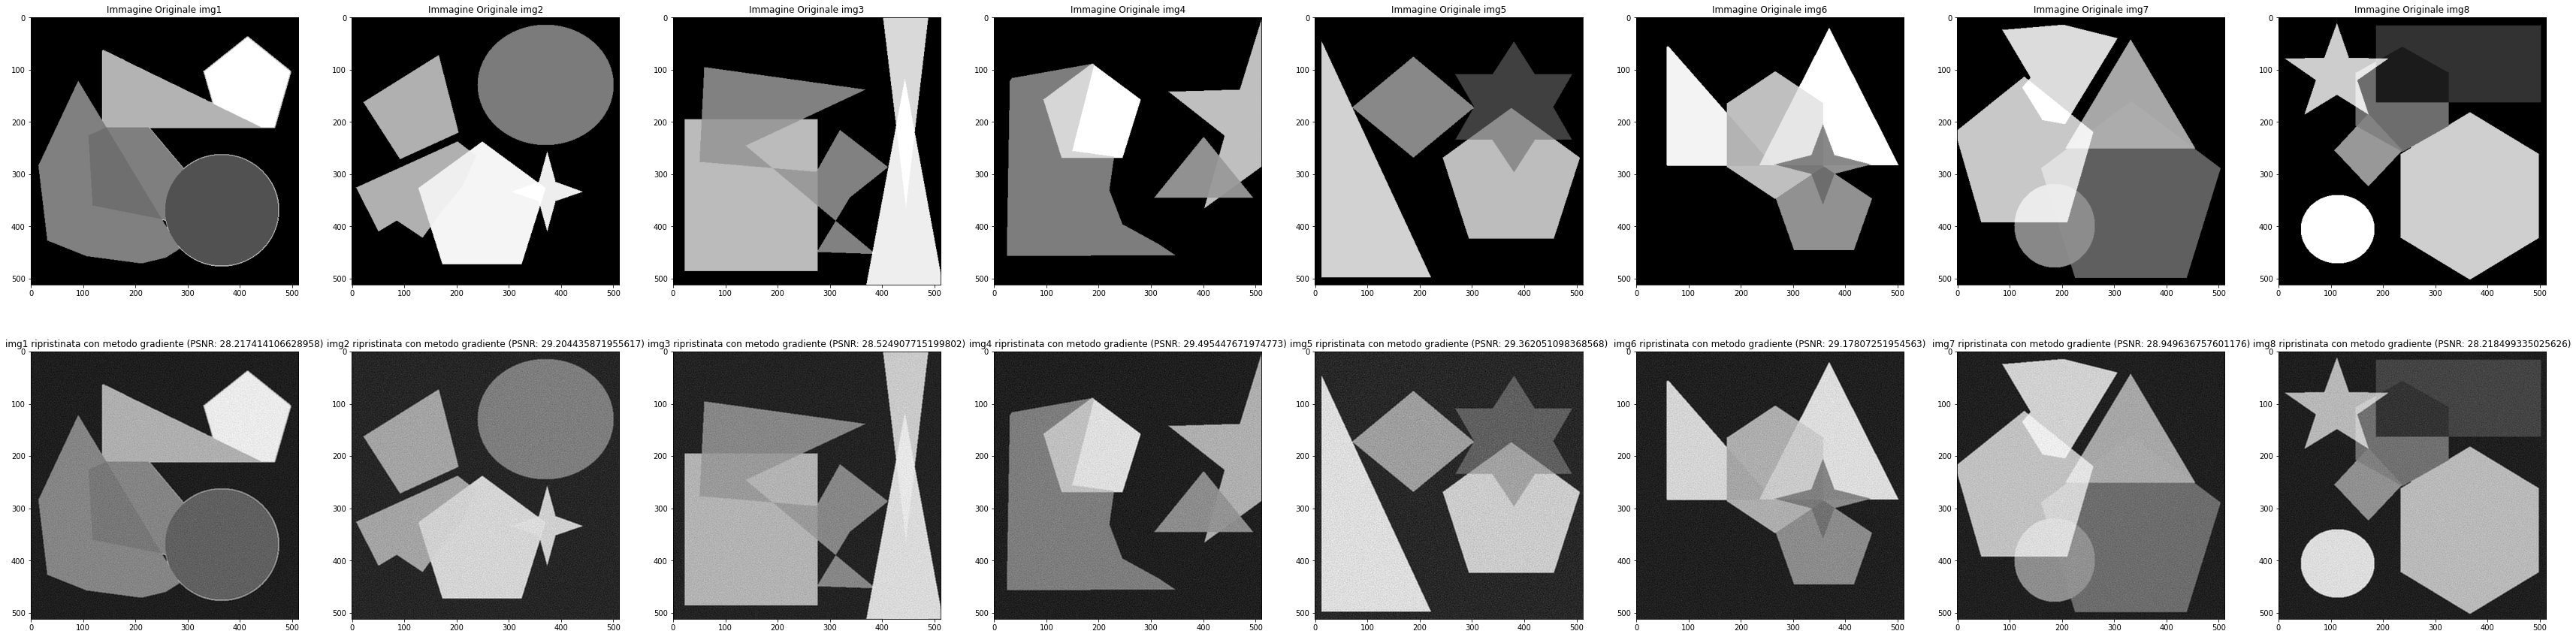
\includegraphics[width=0.9\textwidth]{imgRel/datasetgradiente.png}\label{fig:geomgradiente}
    \caption{Immagini geometriche ripristinate con il metodo del gradiente}
    \end{subfigure}

    \begin{subfigure}{0.5\textwidth}
        \centering
        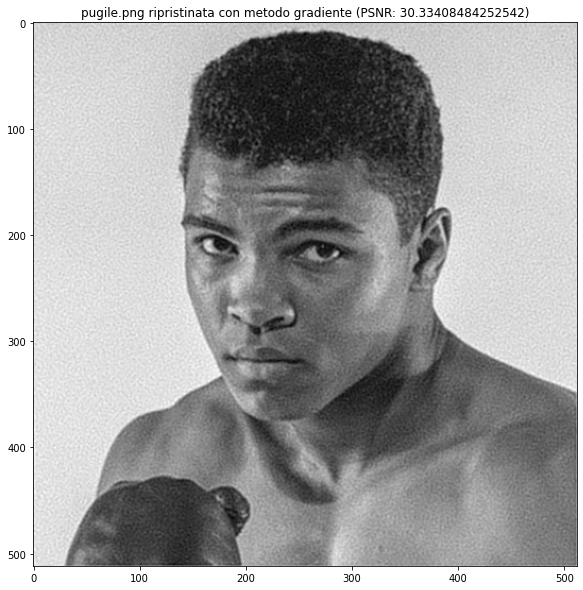
\includegraphics[width=0.6\textwidth]{imgRel/fotogrmg.png}
        \caption{Immagine ritratto ripristinata con il metodo del gradiente}
        \label{fig: pugilemg1}
    \end{subfigure}%
    \begin{subfigure}{0.5\textwidth}\centering
        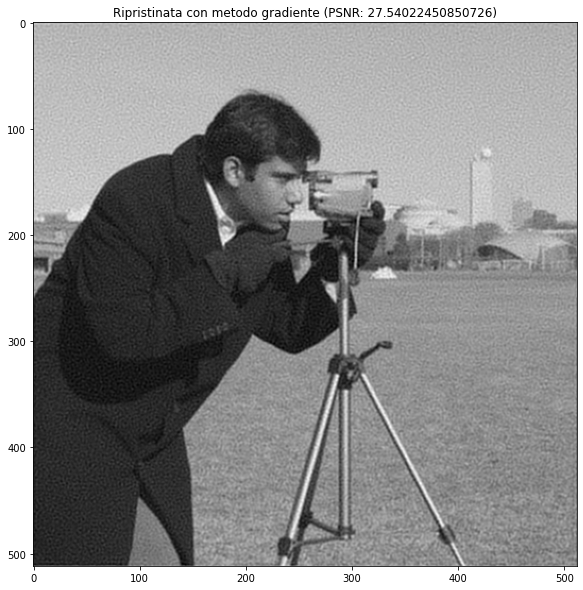
\includegraphics[width=0.6\textwidth]{MANCANTI/cameramanPuntoDueGrad.png}
        \caption{Immagine fotografica ripristinata con il metodo del gradiente}
    \end{subfigure}
\caption{Immagini analizzate ripristinate con il Metodo del Gradiente}
    \begin{minipage}{0.6\textwidth}\centering
        \begin{tabular}{|lcr|}
            \hline
            \rowcolor{orange}
            \multicolumn{1}{|c|}{\textbf{Immagine}} & \multicolumn{1}{l|}{\textbf{PSNR corrotte}} & \multicolumn{1}{c|}{\textbf{PSNR riprist.}} \\ \hline
            img1.png                                & 27.7886                                     & 28.217                                      \\
            img2.png                                & 29.2539                                     & 29.204                                      \\
            img3.png                                & 28.0014                                     & 28.525                                      \\
            img4.png                                & 29.6382                                     & 29.495                                      \\
            img5.png                                & 29.4566                                     & 29.362                                      \\
            img6.png                                & 29.1727                                     & 29.178                                      \\
            img7.png                                & 28.8132                                     & 28.949                                      \\
            img8.png                                & 27.7142                                     & 28.218                                      \\ \hline
            pugile.png                              & 30.3576                                     & 30.334                                      \\
            data.camera()                           & 27.4138                                     & 27.540                                      \\ \hline
            \end{tabular}
        \captionof{table}{Valori PSNR delle immagini ricostruite con il metodo del gradiente}      
    \end{minipage}
\end{figure}

\begin{figure}[H]
    \centering
    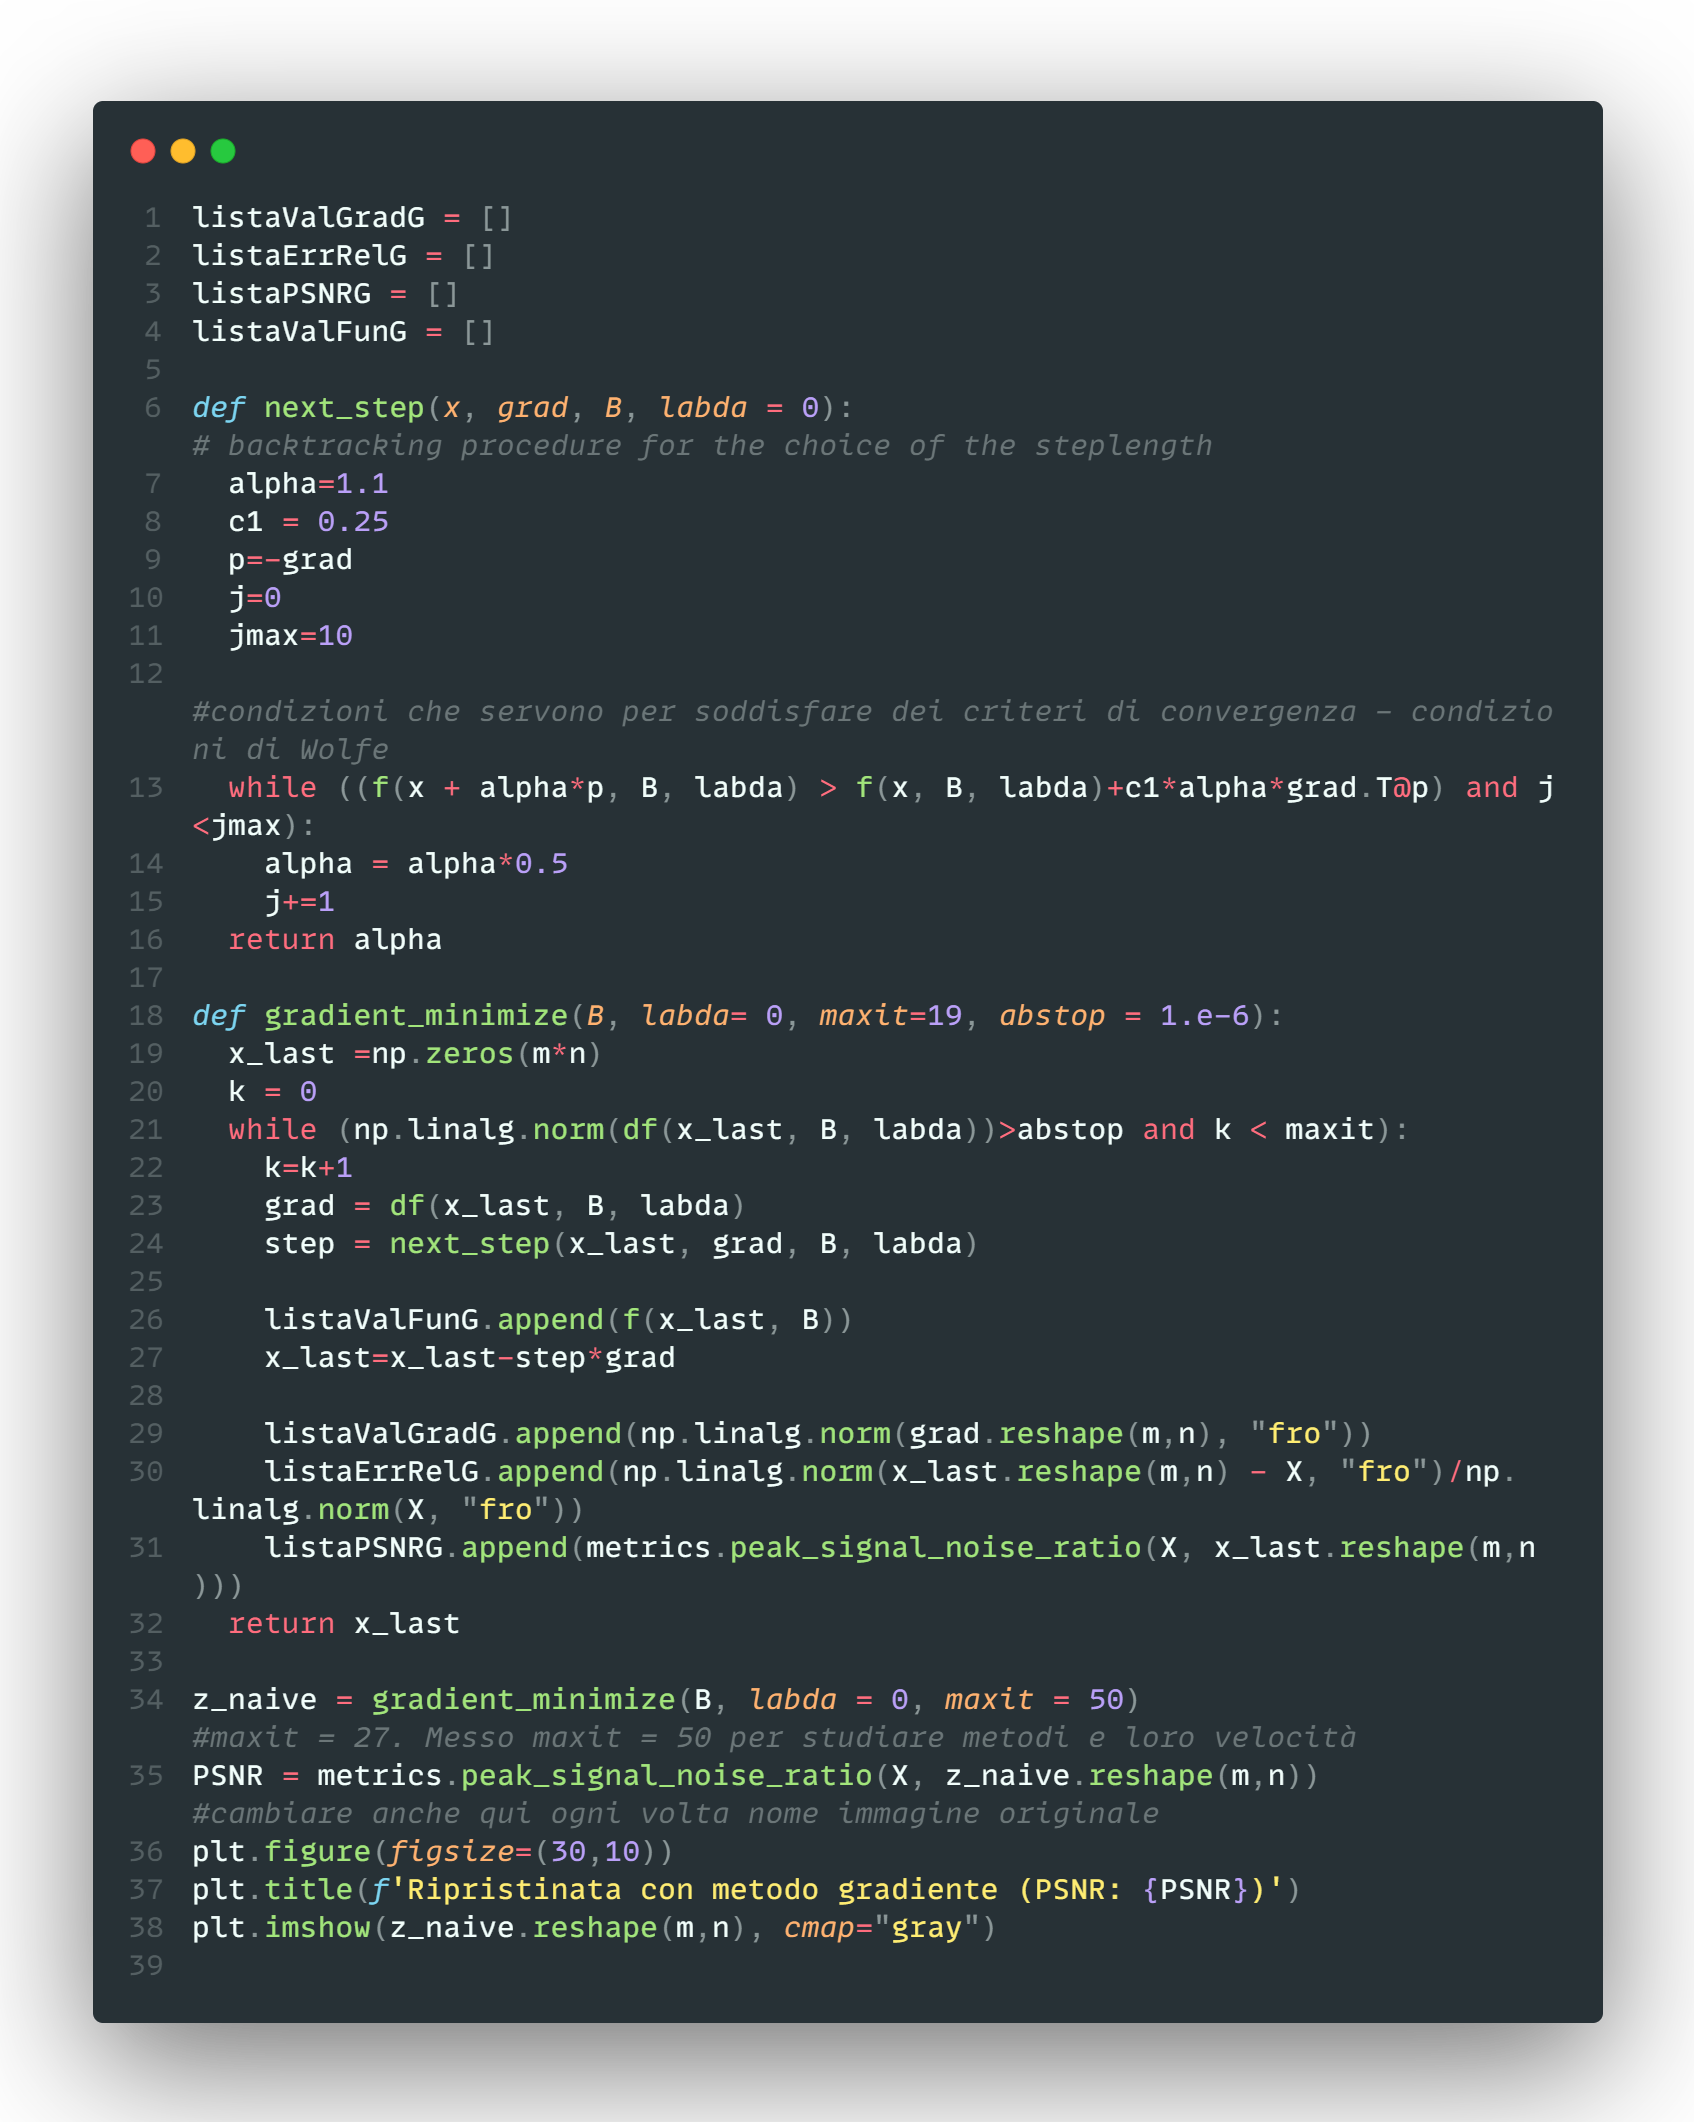
\includegraphics[width=0.7\textwidth]{imgCode/metGrad.png}
    \caption{Codice in \code{Python 3} del metodo del gradiente applicato ad una singola immagine}
\end{figure}
